% !TEX TS-program = pdflatex
% !TEX encoding = UTF-8 Unicode

% This is a simple template for a LaTeX document using the "article" class.
% See "book", "report", "letter" for other types of document.

\documentclass[11pt]{article}

\usepackage[utf8]{inputenc} % set input encoding (not needed with XeLaTeX)

%%% Examples of Article customizations
% These packages are optional, depending whether you want the features they provide.
% See the LaTeX Companion or other references for full information.

%%% PAGE DIMENSIONS
\usepackage{geometry} % to change the page dimensions
\geometry{letterpaper} % or letterpaper (US) or a5paper or....

\usepackage[]{graphicx} % support the \includegraphics command and options

% \usepackage[parfill]{parskip} % Activate to begin paragraphs with an empty line rather than an indent

%%% PACKAGES
\usepackage{booktabs} % for much better looking tables
\usepackage{array} % for better arrays (eg matrices) in maths
\usepackage{paralist} % very flexible & customisable lists (eg. enumerate/itemize, etc.)
\usepackage{verbatim} % adds environment for commenting out blocks of text & for better verbatim
\usepackage{subfig} % make it possible to include more than one captioned figure/table in a single float
% These packages are all incorporated in the memoir class to one degree or another...
\usepackage{mathtools}
\usepackage{listings}
\usepackage{amsmath}
\usepackage{setspace}
\doublespacing
% or:
%\onehalfspacing
%\usepackage[authoryear]{natbib}
\usepackage{hyperref}
\usepackage{float}
\usepackage{epsfig}
\usepackage{import}



%%% HEADERS & FOOTERS
\usepackage{fancyhdr} % This should be set AFTER setting up the page geometry
\pagestyle{fancy} % options: empty , plain , fancy
\renewcommand{\headrulewidth}{0pt} % customise the layout...
\lhead{}\chead{}\rhead{}
\lfoot{}\cfoot{\thepage}\rfoot{}

%%% SECTION TITLE APPEARANCE
\usepackage{sectsty}
\allsectionsfont{\sffamily\mdseries\upshape} % (See the fntguide.pdf for font help)
% (This matches ConTeXt defaults)

%%% ToC (table of contents) APPEARANCE
\usepackage[nottoc,notlof,notlot]{tocbibind} % Put the bibliography in the ToC
\usepackage[titles,subfigure]{tocloft} % Alter the style of the Table of Contents
\renewcommand{\cftsecfont}{\rmfamily\mdseries\upshape}
\renewcommand{\cftsecpagefont}{\rmfamily\mdseries\upshape} % No bold!
\usepackage{datetime}

\newdateformat{mydate}{\monthname[\THEMONTH] \THEYEAR}


\title{THE MILLIMETER-WAVELENGTH SULFUR DIOXIDE ABSORPTION SPECTRA MEASURED UNDER SIMULATED VENUS CONDITIONS }
\author{A Masters Thesis Proposal\\
Presented to\\
The Academic Faculty \\
by \\
Amadeo Bellotti}
\date{\mydate\today} % Activate to display a given date or no date (if empty),
         % otherwise the current date is printed 

\begin{document}
\maketitle

%\begin{abstract}
%The objective of the proposed research is to develop a mathematical model that accurately estimates the opacity of sulfur dioxide in a carbon dioxide atmosphere under conditions characteristic of the Venus troposphere based on extensive laboratory measurements. High precision measurements of the millimeter-wavelength properties of sulfur dioxide are being conducted under multiple pressure and temperatures. These measurements are being conducted in both W-band and F-band (2-3 and 3-4 millimeter-wavelengths). The results of this research will significantly improve the understanding of the millimeter-wavelength emission spectrum of Venus and possibly determine the source of variations in the Venus millimeter-wavelength emissions. 
%\end{abstract}
\newpage
\tableofcontents
\chapter{Introduction}

%\section{Introduction}
Active and passive microwave remote sensing techniques have been extensively used in the study of our sister planet, Venus. Unlike Earth's atmosphere, the Venus atmosphere is mostly comprised of gaseous carbon dioxide (CO$_2$). CO$_2$ comprises 96.5\% of the atmosphere along with gaseous nitrogen (N$_2$) at about 3.5\%. The Venus atmosphere has multiple trace constituents such as sulfur dioxide (SO$_2$), carbon monoxide (CO), water vapor (H$_2$O), carbonyl sulfide (OCS), and sufuric acid vapor (H$_2$SO$_4$) \cite{Suleiman-thesis}.

Two sulfur-bearing compounds dominate the millimeter-wave emission from Venus: sulfur dioxide (SO$_2$) and gaseous sulfuric acid (H$_2$SO$_4$). At higher pressures H$_2$SO$_4$ thermally dissociates, forming H$_2$O and SO$_3$, both of which exhibit relatively small amounts of microwave absorption at the abundance levels present in the Venus atmosphere. Thus, in the deep atmosphere, only SO$_2$ and CO$_2$ have the potential to affect the observed microwave emission.

Utilizing the millimeter-wavelength system at the Planetary Atmospheres Laboratory at Georgia Institute of Technology, it has been possible to simulate the upper troposphere of Venus and take precision measurements of the millimeter-wavelength properties of sulfur dioxide. Using the measurements, a model that accurately predicts the opacity of sulfur dioxide in the Venus atmosphere has been verified. Applying this opacity model to a newly developed radiative transfer model will make it possible to determine the source of variations in the Venus millimeter-wavelength emission, such as were observed by Sagawa \cite{Sagawa-2008}.

\section{Background and Motivation}

Radio absorptivity data from planetary atmospheres can be used to infer abundances of microwave absorbing constituents. Such data is obtained from entry probe radio signal absorption measurements, spacecraft radio occultation experiments, and earth-based or spacecraft based radio emission observations. This can only be done if reliable models for the microwave absorbing properties of potential constituents are available. The use of theoretically-derived microwave absorption properties for such atmospheric constituents, or models based on laboratory measurements taken under environmental conditions different then the atmosphere being studied, often leads to significant misinterpretation of the measured opacity data. Even if laboratory measurements have been already conducted, improvements in the sensitivity of microwave sensors may require higher precision laboratory measurements. 

Using the measured millimeter-wavelength absorption spectra of SO$_2$ in a CO$_2$ atmosphere and the resulting opacity formalism a radiative transfer model (RTM), has now been produced. The model can be applied to earth-based and spacecraft-based radio emission measurements so as to provide planetary maps of SO$_2$ abundances at all altitudes of the Venus atmosphere. %Using this model along with observations from Sagawa \cite{observations} it will be possible to identify vertical abundances of SO$_2$ in different places of the Venus atmosphere. 
This model can be applied to earth based millimeter-wavelength observations of Venus so as to provide planetary maps of sulfuric acid vapor and sulfur dioxide abundances at and immediately below the main cloud layer. Interpretation of such observations will complement the study of long-term variations of SO$_2$ variations at the 70 km altitude level made with Venus-orbiting ultraviolet(uv) spectrometers. 

It is well understood that the microwave emission spectrum of Venus reflects the abundance and distribution of its constituents. The most critical limiting factor in sensing these constituents is the knowledge of there microwave absorption properties under a Venus atmosphere. The millimeter-wavelength absorption spectra of SO$_2$ has been measured by Fahd and Steffes, 1992 \cite{Fahd-thesis}.  Using newer technology it is possible to measure more resonances with higher precision. Improved laboratory capabilities also allow for a wider range of environmental conditions, similar to those actually being probed, to be simulated. The millimeter-wavelength system used is able to reproduce conditions similar to those that exist on Venus. The centimeter-wave absorption spectra already measured by Steffes et al. 2014 \cite{Steffes-2014} has been used to help choose a model that best represents the centimeter and millimeter wavelength opacity of SO$_2$ in a CO$_2$ atmosphere. 

Sagawa (2008) attributes the Venus millimeter-wavelength continuum brightness variations to spatial variations in the abundances of both gaseous H$_2$SO$_4$ and SO$_2$ just below the cloud layer (48 km altitude). The developed RTM's weighting function confirms these results. Sagawa has also suggested that the effects of both constituents can be distinguished based on differences in frequency dependencies of their millimeter-wavelength opacities. However, to accomplish this, high accuracy models must be developed that characterize the opacity of each constituent and its frequency dependence. This thesis successfully characterizes SO$_2$'s absorption as a function of pressure, temperature, concentration, and frequency for both centimeter and millimeter-wavelengths. 


\section{Organization}
The objective of this research has been to determine the absorption properties of gaseous sulfur dioxide in a carbon dioxide atmosphere at millimeter wavelengths. The formalism identified from the results has been used to create a radiative transfer model (RTM) for Venus. The thesis is organized as follows:
\\ \\
\noindent Chapter 2 provides a discussion of the theory behind measuring the millimeter-wavelength opacity of a gas. A complete description of the measurement system used for this work is presented.
\\ \\
\noindent Chapter 3 describes the measurement uncertainties involved with the experimental setups. An explanation of the data sets used and the analysis process are included. Finally a suggested model is presented.
\\ \\
\noindent Chapter 4 describes the radiative transfer model created from this work. A discussion on radiative transfer theory is presented followed by describing the necessary parameters. The correct formula for tracing a ray through different atmospheric layers as well as methods for making the RTM computationally efficient follows. Later there is a discussion on how to integrate a simulated antenna beam pattern into this RTM to simulate an antenna beam. Ending this chapter is the model's results compared to Venus observations.
\\ \\
\noindent Chapter 5 summarizes the results of this work and presents suggestions for further investigations. An overview on this work's impact on Venus Observations is provided.

\chapter{Theoretical Basis and Previous Work}

\section{Physical Structure of SO$_2$}
\section{Physical Structure of CO$_2$}
\section{Van Vlevk and Weisskopf Model}
\chapter{Experiment Design, Theory, and Results}

Verifying the millimeter-wavelength absorption spectrum of SO$_2$ is important for the study of the atmosphere of Venus. Making measurements under simulated Venus conditions assures the accuracy of any model derived from such measurements.
 We describe the theory, laboratory equipment, measurement procedure, and derived uncertainties in the measurements of the millimeter-wavelength absorptivity of gaseous sulfur dioxide under simulated Venus conditions.

\section{Measurement Theory}

In this experimental program, the quality factor (Q) of a resonant mode of a resonator is used to measure the absorption of a gas or gas mixture \cite{Hanley-2007}. The quality factor of a resonance is given by \cite{Matthaei-1980}

\begin{equation} \label{eq:qlong}
Q = \frac{2\pi f_0 \textnormal{ x Energy Stored}}{\textnormal{Average Power Loss}}
\end{equation}

\noindent where $f_0$ is the resonant frequency. The Q of a resonance can be measured directly from $f_0$ by dividing it by its half-power bandwidth (HPBW).

\begin{equation} \label{eq:qshort}
Q = \frac{f_0}{HPBW}
\end{equation}

\noindent The Q of a lossy gas ($\epsilon'/\epsilon''$) and its opacity are related by
\begin{equation} \label{eq:alphaapprox}
\alpha \approx \frac{\epsilon'' \pi}{\epsilon' \lambda} = \frac{1}{Q_{gas}} \frac{\pi}{\lambda}
\end{equation}

\noindent where $\epsilon'$ and $\epsilon''$ are the real and imaginary permittivity of the gas, $\lambda$ is the wavelength in km, and $\alpha$ is the absoptivity of the gas in Nepers/km (1 Neper = 8.686 dB). Since Q can be affected by more than just the gas added, the Q of the gas-filled resonator is given by

\begin{equation} \label{eq:qloaded}
\frac{1}{Q_{loaded}^m} = \frac{1}{Q_{gas}} + \frac{1}{Q_{r}} + \frac{1}{Q_{ext1}} +\frac{1}{Q_{ext2}}
\end{equation}

\noindent where $Q_{loaded}^m$ is the measured quality factor of a resonance in the presence of a test gas, $Q_{gas}$ is the quality factor of the gas under test, $Q_{r}$ is the quality factor of the resonator in the absense of coupling losses, and $Q_{ext1}$ and $Q_{ext2}$ are the external coupling losses. Since the resonator used is symmetric, it is safe to assume $Q_{ext1} = Q_{ext2}$. Coupling losses can be derived from the transmissivity $t = 10^{-S/10}$, where $S$ is the measured insertion loss of the resonator in decibels (dB) at the frequency of a particular resonance using the following relationship \cite{Matthaei-1980}

\begin{equation} \label{eq:t}
t = \left[ 2 \frac{Q^m}{Q_{ext}} \right]^2,
\end{equation}

\begin{equation} \label{eq:qext}
Q_{ext} = \frac{2Q^m}{\sqrt{t}}
\end{equation}

\noindent $Q_r$ is related to the measured Q at a vacuum by

\begin{equation}\label{eq:qvac}
\frac{1}{Q_{vac}^m} =  \frac{1}{Q_{r}} + \frac{1}{Q_{ext1}} +\frac{1}{Q_{ext2}}
\end{equation}

\noindent where $Q_{vac}^m$ is the measured Q under vacuum conditions. Substituting equation \ref{eq:qext} into equations \ref{eq:qloaded} and \ref{eq:qvac} gives

\begin{equation}\label{eq:qgas}
\frac{1}{Q_{gas}} = \frac{1 - \sqrt{t_{loaded}}}{Q^m_{loaded}} - \frac{1-\sqrt{t_{vac}}}{Q_{vac}^m}
\end{equation}

\noindent where $t_{loaded}$ and $t_{vac}$ are the transmissivity of the resonance taken in loaded and vacuum conditions respectively. When gas is added to the resonator there is a shift in the center frequency corresponding to the refractive index of the test gas. Since the quality factor is reliant on the center frequency this will affect the comparison between the two measurements, even if the gas being tested is lossless. This effect is called dielectric loading \cite{Deboer-1993}. This effect can be corrected by performing additional measurements of the quality factor with a lossless gas present. Adding the lossless gas shifts the center frequency of the resonances, and by adding more or less gas the center frequency can be adjusted to be exactly the same as the lossy gas. These measurements are used in place of the vacuum measurements in equation \ref{eq:qgas} and by converting Nepers/km to dB/km equation \ref{eq:alphaapprox} becomes

\begin{equation} \label{eq:alphamatch}
\alpha = 8.686 \frac{\pi}{\lambda}\left(\frac{1 - \sqrt{t_{loaded)}}}{Q^m_{loaded}} - \frac{1-\sqrt{t_{matched}}}{Q_{matched}^m} \right) dB/km
\end{equation}

\section{Millimeter-Wavelength Measurement System}

The high-sensitivity millimeter-wavelength system used for measuring the opacity of gaseous sulfur dioxide under Venus conditions is similar to the one used by Devaraj and Steffes \cite{Devaraj-2011} \cite{Devaraj-thesis}. The system is comprised of two subsystems for measuring different bands of the millimeter-wavelength spectrum (W-band/F-band). The simulator consists of a glass pressure chamber capable of withstanding up to 3 bars of pressure along with a temperature chamber capable of operating up to 400 K. The W-band subsystem is used for measurements in the 2.7-4.0 millimeter-wavelength range while the F-band system is used for the 2-3 milimeter-wavelength range. The following sections describe each subsystem and their components. 

\subsection{W-band Subsystem}

The W-band measurement system is used to measure the 2.7-4.0 mm-wavelength properties of sulfur dioxide and shown in Figure \ref{fig:wbandimage}.

A synthesized swept signal generator (HP 83650B) is used to generate a signal in the 12.5-18.3 GHz range which is fed to a times-six active multiplier chain (AMC) via low-loss, high frequency coaxial cables. The active multiplier then feeds the 75-110 GHz signals (swept over the range covered by each single resonance) to the Fabry-Perot resonator via WR-10 waveguides. The millimeter-wavelength radio frequency (RF) signal from the output port of the Fabry-Perot resonator (FPR) is fed via waveguide to a QuinStar Technology QMH series harmonic mixer. The local oscillator (LO) and the intermediate frequency (IF) are connected via an external diplexer. The harmonic mixer is locked to the 18th harmonic of the spectrum analyzer LO and is used in the ``external mixer'' mode with the spectrum analyzer (HP 8564E). 

\begin{figure}[H]
    \centering
	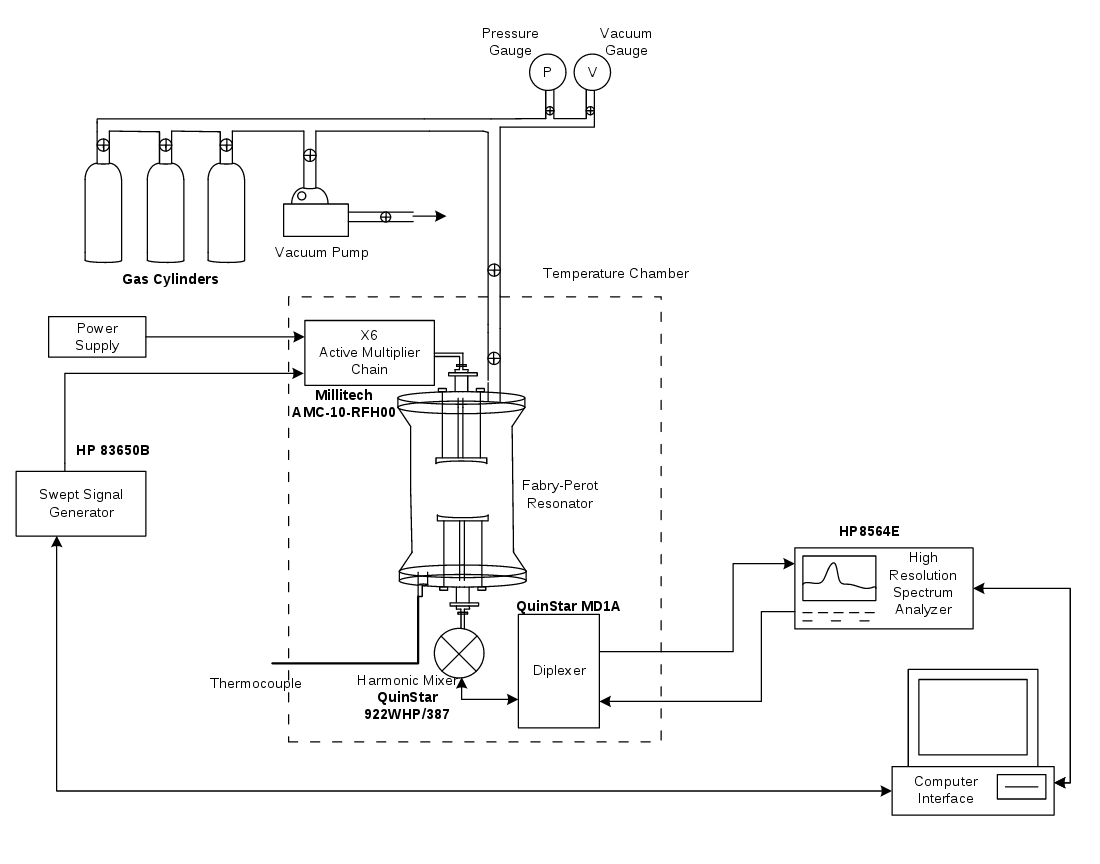
\includegraphics[width=1\textwidth]{./images/w-bandsystem.png}
	\caption{Block diagram of the W-band measurement system. Solid lines represent the electrical connections and the arrows show the direction of the signal propagation. Valves controlling the flow of gasses are shown by small crossed circles.}
    \label{fig:wbandimage}
\end{figure}


\subsection{F-band Subsystem}
The F-band measurement system is used to measure the 2-3 mm-wavelength properties of sulfur dioxide and is shown in figure \ref{fig:fbandimage}.

The swept signal generator (HP 83650B) is used to generate a signal in the 33-50 GHz range which
is amplified and fed through a frequency tripler. The output of the tripler is fed to the input of the FPR via WR-8 waveguides. The RF signal from the output port of the FPR is fed to a harmonic mixer which can operate with an LO frequency as high as 18 GHz. An external diplexer is used to combine the IF and LO signals. For a particular RF and IF frequency,  the LO frequency can be computed using

\begin{equation} \label{eq:fbandlo}
f_{LO} = \frac{f_{RF} - f_{IF}}{N_H	}
\end{equation}

\noindent where N$_H$ is the lowest integer such that $f_{lo} < 18$ GHzs.

\begin{figure}[H]
    \centering
	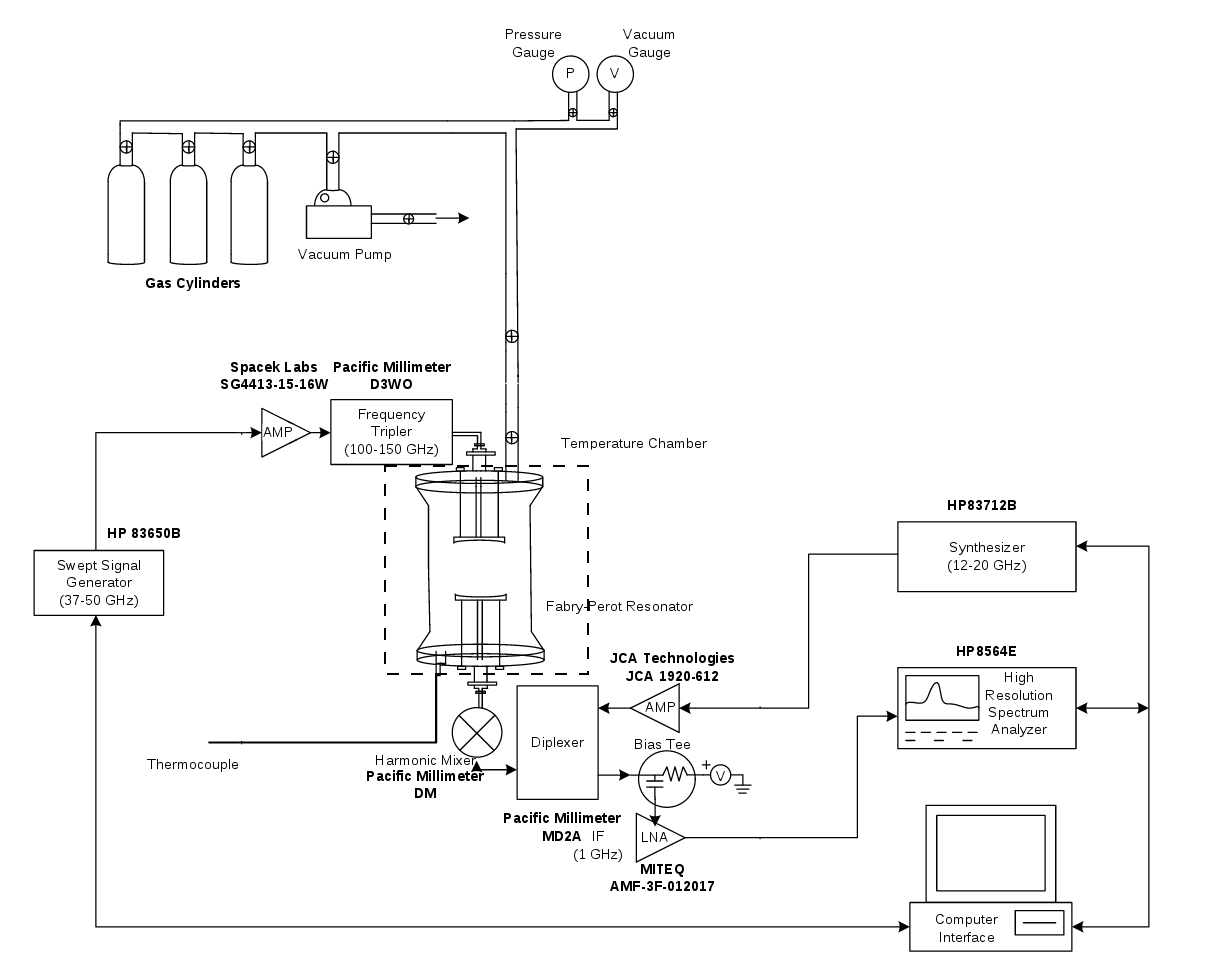
\includegraphics[width=1\textwidth]{./images/f-bandsystem.png}
	\caption{Block diagram of the F-band measurement system. Solid lines represent the electrical connections and the arrows show the direction of the signal propagation. Valves controlling the flow of gasses are shown by small crossed circles.  }
    \label{fig:fbandimage}
\end{figure}

\section{Data Handling Subsystem}

The data acquisition system consists of a computer connected to the spectrum analyzer (HP 8564E), swept signal generator (HP 83650B), and continuous wave (CW) signal generator (HP 83712B, the local oscillator for the F-Band system) via a general purpose interface bus (GPIB). The instruments are controlled via Matlab script and their appropriate programming language. The software used is similar to Devaraj and Steffes \cite{Devaraj-thesis, Devaraj-2011} with modifications for equipment changes.

\section{Measurement Procedure}

The most important prerequisite for performing measurement of gas properties is ensuring a leak-proof system. This is done through two methods, the first method is by drawing a vacuum inside the FPR and verifying the integrity of the vacuum over time. The second method is by adding a positive pressure of CO$_2$ to the system and making sure there are no leaks in any of the connectors and valves. Ensuring a leak-proof system allows for not only precise measurements but also ensures no toxic gases are released into the testing environment.

After the system is ensured to be leak-proof and at a stable temperature, a vacuum is drawn and a measurement is taken using the appropriate subsystem (W-band for 2.7-4.0 mm-wavelengths, F-band for 2-3 mm-wavelengths). This allows for a baseline measurement of the FPR's resonances and the Quality factor. Once this baseline is established the gas under test is added to the system.

Once the gas temperature has stabilized, another set of tests measuring the resonant frequencies along with the quality factors is taken. More gas is added and the procedure is repeated until measurements at all suitable pressures are taken. A vacuum is drawn once again but this time it is pumped overnight due to the possibility of adsorption (or ``sticking'') of the gas being tested (SO$_2$) to metal surfaces inside the vessel. This second vacuum measurement is taken to measure any possible system drift.

Once the second vacuum measurement is taken, CO$_2$ is then added to the chamber until the resonances are matched to the same frequency of our test gas (note that at the pressures and frequencies used for our experiment, pure CO$_2$ is essentially lossless). Again measurements are taken and this is repeated for every pressure of the test gas. Once completed a vacuum is again drawn and another test is taken. 

Lastly the system is set up for a transmissivity test where we measure t (equation \ref{eq:t}) for each given resonant frequency. This is done by by passing the Fabry-Perot resonator and connecting the input and output waveguides through a WR-10 20 dB directional coupler. The signal level is then measured and used to calculate t.  The system is then set back up and is ready for a new test. %Reference table \ref{tab:testmatrix} for the testing matrix being used.


%\section{Preliminary Results}

Currently the millimeter-wavelength system is completely operational in the Planetary Atmospheres Laboratory at The Georgia Institute of Technology. Using this system, high precision measurements of SO$_2$'s millimeter-wavelength absorption have recently been completed as part of this work. A preliminary model of SO$_2$'s absorption properties is available from Suleiman's previous work on microwave laboratory measurements \cite{Suleiman-thesis}. Additionally measurements  of SO$_2$'s centimeter-wavelength absorption have recently been taken under deep Venus conditions \cite{so2-cent-lab} \cite{so2-cent-model}. 

\subsection{Millimeter-Wavelength Results}

Only one previous measurement of SO$_2$'s mm-wavelength opacity under Venus simulated conditions has been done (see Fahd et. al. 1991) \cite{fahd-so2} This measurement was done using only one frequency (94.1 GHz) in the mm-wavelength spectra.

In our experiment, eight different frequencies have been already tested using the millimeter-wavelength system measuring 100 mbar of SO$_2$ along with separate tests at 1 bar CO$_2$ combined with the SO$_2$  and 2 bar of CO$_2$ combined with the SO$_2$. This allows for a comparison with Fahd's model and with Suleiman's model at higher frequencies.  

\subsubsection{Absorption Model}

The goal of the laboratory measurements is to create a mathematical model that accurately estimates the opacity of sulfur dioxide in a carbon dioxide atmosphere under all possible conditions of temperature, pressure, concentration, and frequency (fTPC space). For the data fitting process we will use data taken with the FPR along with data from the Planetary Atmospheres Laboratory centimeter-wavelength system  \cite{so2-cent-lab} \cite{so2-cent-model} to create a model that best fits the fTPC space. 

Extrapolating models for SO$_2$'s absorption into the mm-wavelength allows for a good starting point in the model creation process. As visible in the following figures, the absorption model matches the same shape as previous models but is lower by about 20\%. Finding a unified model for SO$_2$'s absorption will compensate for this change.

Figures \ref{fig:so2-116}, \ref{fig:so2-943}, and \ref{fig:so2-1987} show the initial data taken for SO$_2$ opacity in the 3-4 mm-wavelength range. It is clear that previous absorption models work well in predicting the shape of the millimeter-wavelength absorption spectrum of SO$_2$.

\begin{figure}[H]
    \centering
	\includegraphics[width=0.8\textwidth]{./plots/35C_W_High/{0.116-modelComparison}.eps}
	\caption{Measured absorption spectrum given 116 mbar of SO$_2$ at 308K in the W-band range. Shown for comparison are models from Devaraj (2011), Suleiman et al (1996), and Fahd and Steffes (1992).}
    \label{fig:so2-116}
\end{figure}

\begin{figure}[H]
    \centering
	\includegraphics[width=0.8\textwidth]{./plots/35C_W_High/{0.943-modelComparison}.eps}
	\caption{Measured absorption spectrum given 116 mbar of SO$_2$ and 827 mbar of CO$_2$ at 308K in the W-band range.
	Shown for comparison are models from Devaraj (2011), Suleiman et al (1996), and Fahd and Steffes (1992).}
    \label{fig:so2-943}
\end{figure}

\begin{figure}[H]
    \centering
	\includegraphics[width=0.8\textwidth]{./plots/35C_W_High/{1.987-modelComparison}.eps}
	\caption{Measured absorption spectrum given 116 mbar of SO$_2$ and 1871 mbar of CO$_2$ at 308K in the W-band range.
	Shown for comparison are models from Devaraj (2011), Suleiman et al (1996), and Fahd and Steffes (1992).}
    \label{fig:so2-1987}
\end{figure}
\chapter{Model Fitting and Modifications}
In total, 36 data sets were taken (12 at \textasciitilde 308 K and 24 at \textasciitilde 343 K) at 2-4 mm-wavelength. This along with data taken at the centimeter-wavelength by Steffes et al. 2014 \cite{Steffes-2014}(10 data sets at \textasciitilde 435 K, 10 data sets at \textasciitilde 490 K, and 5 data sets at \textasciitilde 550 K) where used in finding the best-fit model.

Before creating a new formalism for the absorption of SO$_2$ in a CO$_2$ atmosphere analysis of previous models are done. The Van Vlevk and Weisskopf Model as done by Fahd and Steffes \cite{Fahd-thesis} with the new rotational line catalog (VVW) was found to fit 85.88\% of all 500 within $2\sigma$ uncertainty. Consideration of the model analysis process and the final model are presented.
\section{Measurement Uncertainties}

There are five uncertainties for any absorptivity measurements using the centimeter and millimeter wavelength system: instrumentation errors and electrical noise ($Err_{inst}$), errors in dielectric matching ($Err_{diel}$), errors in transitivity measurement ($Err_{trans}$), errors due to resonance asymmetry ($Err_{asym}$), and errors in measurement conditions ($Err_{cond}$) resulting from uncertainties in temperature, pressure, and mixing ratio. The term $Err$ is used for representing uncertainties instead of the more frequently used $\sigma$ to avoid confusion between $1\sigma$,$2\sigma$, and $3\sigma$ uncertainties.

Instrumental errors and electrical noise are caused due to the sensitivity of the electrical devices and their ability to accurately measure bandwidth ($BW_{measured}$) and the center frequency ($f_o$). Electrical noise arises from the frequency references and the noise of the internal electronics. Since electrical noise is uncorrelated, it's best estimate of the uncertainty is the mean of multiple measurements. The variance of the best error estimate is given by the sample variance ($S^2_N$) weighted by the confidence coefficient ($B$) as
\begin{equation}\label{eq:sigman}
\sigma^2_N = B \frac{S^2_N}{N_{samples}}
\end{equation}

\noindent where $N_{samples}$ is the number of independent measurements of the sample. For the millimeter-wavelength system, five sets of independent measurements of each resonance are taken. A confidence coefficient ($B$) of 2.776 is used. This corresponds to the 95\% confidence interval. The center frequency standard deviation is very small and its effect on the uncertainty in $Q$ is negligible. Therefore, $S_N$ i the sample standard deviation of the bandwidth of the measurements.

The HP 8564E spectrum analyzer is used for measuring the resonances in the millmeter-wavelength system. It's manufacturer specified instrumental uncertainties are the $3\sigma$ values \cite{Hewlett-Packard}. The $3\sigma$ standard deviation for the center frequency and bandwidth are estimated by 

\begin{equation}\label{eq:sigmao}
Err_o \leq \pm (f_o \times f_{ref\:acc} + 0.05 \times SPAN + 0.15 \times RBW +10 ) (Hz)
\end{equation}
\begin{equation}\label{eq:sigmabw}
Err_{BW} \leq \pm (BW_{measured} \times f_{ref\;acc} + 4 \times N_H +2 \times LSD ) (Hz)
\end{equation}

\noindent where $f_{ref\;acc}$ is given as

\begin{equation}\label{eq:frefacclong}
\begin{split}
f_{ref\;acc} = (aging \times {time\;since\;calibration}) + {inital\;achievable\;accuracy} \\
+ {temperature\;stability}
\end{split}
\end{equation}

\noindent and $f_o$, SPAN, RBW, $N_H$, and LSD are the center frequency, frequency span, resolution bandwidth, harmonic number, and least significant digit of the bandwidth measurement, respectively. LSD is calculated as $LSD = 10^x$ for the smallest positive integer value of x such that SPAN $< 10^{x+4}$. For SPAN $\leq 2$ MHz$\times N_h$, the SPAN multiplication factor of 0.05 is replaced with 0.01. For the spectrum analyzer used, $f_{ref\;acc}$ reduces to

\begin{equation}\label{eq:frefacc}
f_{ref\;acc} = (10^{-7} \times {years\;since\;calibrated}) + 3.2\times 10^{-8}
\end{equation}

The worst case scenario is used to transform the uncertainty in center frequency and bandwidth for both loaded and dielectrically matched measurements into an uncertainty in absorptivity as described in DeBoer and Steffes \cite{DeBoer-Steffes}.

\begin{equation}
Err^2_\Psi = \langle {F_l^2}\rangle + \langle {F_m^2}\rangle -\langle {F_l F_m}\rangle
\end{equation}

\noindent where
\begin{equation}
\langle {F_i^2}\rangle = \frac{\Upsilon_i^2}{f_{oi}^2}
\left[ \frac{Err_o^2}{Q_l^2} + Err_{BW}^2 + Err_{Ni}^2 + \frac{2Err_o Err_{BW}}{Q_i} \right], i= l,m
\end{equation}
\begin{equation}
\langle {F_l F_m}\rangle = -\frac{\Upsilon_l \Upsilon_m}{f_{ol} f_{om}}
\left[ \frac{Err_o^2}{Q_i Q_m} + Err_{BW}^2 + \frac{Err_o Err_{BW}}{Q_l} + \frac{Err_o Err_{BW}}{Q_m}\right]
\end{equation}
\begin{equation}
Q_i = \frac{f_{oi}}{f_{BWi}}, i = l,m
\end{equation}
\begin{equation}
\Upsilon_i = 1- \sqrt{t}, i = l,m
\end{equation}
where $l,m$ denote loaded and dielectrically matched cases, respectively and $f_{ol,om}$ and $f_{BWl,BWm}$ represent center frequency and bandwidth of loaded and dielectrically matched cases respectively. The $2\sigma$ uncertainty of the measured gas absorption due to instrumental errors and electrical noise is given by
\begin{equation}
Err_{inst} = \pm \frac{8.686\pi}{\lambda}Err_\Psi\;(dB/km)
\end{equation}
where $\lambda$ is the wavelength in km. 

Errors in dielectric matching occur when the when the center frequency of the matched measurements are not precisely aligned with the center frequency of the loaded measurement. Since the Q of the resonator can vary slightly this causes an uncertainty in the Q of the matched measurement at the true center frequency of the loaded measurement. The method used to calculate the magnitude of this effect is similar to Devaraj \cite{Devaraj-thesis}. While this error is the most trivial due to the high precision of the software controlled matching it is important to calculate and account for.The magnitude of this effect is calculated by comparing the Q of the three vacuum measurements to that of the dielectric matched measurements

\begin{equation}
\left(\frac{dQ}{df} \right)_i = \left|\frac{Q_{vac,i} - Q_{matched,i}}{f_{vac,i} - f_{matched,i}} \right| \textnormal{ for } i = 1,2,3
\end{equation}

The maximum of the three values is used to calculate a $dQ$ value

\begin{equation}
dQ = \left(\frac{dQ}{df} \right)_{max} \times |f_{loaded} - f_{matched}|
\end{equation}
where $f_{loaded}$ and $ f_{matched}$ are the center frequencies of the resonances under loaded and matched conditions. The error in absorbtivity due to imperfect dielectric matching is then computed by propagating $\pm dQ$ through Equation \ref{eq:alphamatch}.
% \times \left| \left( \frac{1-\sqrt{t_{loaded}}}{Q^m_{loaded}} - \frac{1-\sqrt{t_{matched}}}{Q^m_{matched} + dQ} \right) \left|
\begin{equation}
\begin{split}
Err_{diel} &= \frac{8.686 \pi}{\lambda} 
\\ &\times \left| \left( \frac{1-\sqrt{t_{loaded}}}{Q^m_{loaded}} - \frac{1-\sqrt{t_{matched}}}{Q^m_{matched} + dQ} \right) - \left( \frac{1-\sqrt{t_{loaded}}}{Q^m_{loaded}} - \frac{1-\sqrt{t_{matched}}}{Q^m_{matched} - dQ} \right) \right|\\
 &(dB/km)
\end{split}
\end{equation}

Transmissivity errors are due to the uncertainties in the measurement amplitude. This is caused by loss in the millimeter-wavelength instruments (signal generators and spectrum analyzer), cables, adapters, and waveguides used in this system. Measuring this is done taking multiple tests of the system without the FPR and finding the standard deviation ($S_N$) and weighing it by it's confidence coefficient
\begin{equation}
Err_{msl} = \frac{4.303}{\sqrt{3}}S_N
\end{equation}

For the millimeter-wavelength system, the signal level measurements involve sampling the RF power with a WR-10 20 dB directional coupler to feed the harmonic mixer for down-conversion and detection. While this ensures that the input to the harmonic mixer does not exceed its maximum allowed input power of -10 dBm, the WR-10 does not uniformly sample the input signal throughout the entire frequency range. To compensate for this an aditional 1.5 dB uncertainty is added to insertion loss error. The signal generator has a temperature stability of 1 dB/$10^\circ$ C, but an internal temperature equilibrium is reached after two hours \cite{Hewlett-Packard}. Since the measurements units are stored at a constant temperature this uncertainty can be disregarded. The total uncertainty in insertion loss for the millimeter-wavelength system is calculated by
\begin{equation}
Err_{ins\;loss} = Err_{msl} +1.5\;(dB)
\end{equation}

The error in insertion loss is used to compute the transissivity error
\begin{equation}
Err_{t,i} = \frac{1}{2} ( 10^{-S_i - Err_{ins\;loss}} - 10^{-S_i + Err_{ins\;loss}}) , i=l,m
\end{equation}
where l,m are the loaded and matched cases, respecivey, and S is the insertion loss of the resonator. This is used to compute the $2\sigma$ uncertainties in opacity and is expressed as
\begin{equation}
\begin{split}
Err_{trans} &= \frac{8.686 \pi}{2\lambda}\\ 
 &\times \left| \left( \frac{\sqrt{t_l + Err_{t,l}}- \sqrt{t_l - Err_{t,l}}}{Q^m_{loaded}} - \frac{\sqrt{t_m - Err_{t,m}}- \sqrt{t_m + Err_{t,m}}}{Q^m_{matched}} \right) \right|\\
 &(dB/km).
\end{split}
\end{equation}

Errors from asymmetry are due to the asymmetric nature of the resonances. These are more prominent at low temperatures and short wavelength. Errors due the asymmetry results from the disproportionate asymmetric broadening of the loaded measurements compared to the matched measurements. Equivalent full bandwidths based on assuming symmetry of the high and low sides of the resonances are calculated as
\begin{equation}
BW_{high} = 2 \times (f_{high} - f_{center})
\end{equation}
\begin{equation}
BW_{low} = 2 \times (f_{center} - f_{low})
\end{equation}
where $BW_{high}, BW_{low}, f_{high}, f_{center}$, and $f_{low}$ are the high bandwidth, low bandwidth, higher frequency half power point, center frequency, and lower frequency half power point, respectively. The difference between the opacities calculated using $BW_{high}$ and $BW_{low}$ is defined as $Err_{asym}$ and is calculated by
\begin{equation}
\begin{split}
Err_{asym} &= \frac{8.686 \pi}{\lambda} 
\\ &\times \left| \left( \frac{1-\sqrt{t_{loaded}}}{Q^m_{loaded,high}} - \frac{1-\sqrt{t_{matched}}}{Q^m_{matched,high}} \right) - \left( \frac{1-\sqrt{t_{loaded}}}{Q^m_{loaded,low}} - \frac{1-\sqrt{t_{matched}}}{Q^m_{matched,low}} \right) \right|\\
 &(dB/km)
\end{split}
\end{equation}
Where $Q^m_{matched,high/low}$ and $Q^m_{loaded,high/low}$ are the measured Qs evaluated using the high and low bandwidths for loaded and matched cases. 

The measured uncertainties in temperature, pressure, and concentration in the millimeter-wavelength system contribute to the total uncertainties due to the measurement conditions ($Err_{cond}$). While this does not affect the measurements it still needs to be accounted for during the creation of the models for opacity based on experimental data. It is computed by
\begin{equation}
Err_{cond} = \sqrt{Err_{temp}^2 + Err_{p}^2 + Err_{c}^2 + Err_{leak}^2} (dB/km)
\end{equation}
with $Err_{temp}^2, Err_{p}^2 $, $ Err_{c}^2$, and $Err_{leak}$ representing the 2$\sigma$ uncertainties in the proposed opacity model corresponding to the uncertainties in temperature, pressure, concentration, and leakage. 

Measuring temperature was done using a T type thermocoupler along with a Wavetek 23XT voltmeter. The voltmeter has a temperature accuracy of $\pm (1\% + 2^\circ C)$. Since the voltmeter has a Cold Compensation circuitry it is unnecessary to modify the temperature read from ambient. Also since a test takes an hour to run the temperature drift is insignificant. The uncertainty in temperature reading is calculated by
\begin{equation}
T = T_{read} \pm ( T_{read} \times 1\% + 2)
\end{equation}
Where $T_{read}$ is the temperature readout from the Voltmeter.

Pressure was measured using an Omega DPG-7000 which has an accuracy of $\pm 0.05\%$FS. Since this pressure gauge measures pressure relative to ambient it is necessary to take a measurement before and after each test. The average change in pressure during a test was at most 2 mbar. The way a vacuum was measured was by comparing the Omega DPG-7000 reading to that of an absolute pressure gauge (Druck DPI 104). The Druck has an accuracy of $\pm 0.05\%$FS as well but a resolution of $\pm 1$ mbar. The uncertainty in pressure reading is calculated by
\begin{equation}
P = P_{read} \pm ( P_{FS} \times .05\% + 3)
\end{equation}
Where $P_{FS}$ is the Full Scale pressure of the Omega DPG-7000.

Since $Err_{cond}$ is dependent on the opacity model, this uncertainty is maintained separately from $Err_{tot}$. Thus the total 95\% confidence for the measurement uncertainty is expressed in dB\/km as per Hanley \cite{Hanley-thesis}
\begin{equation}
Err_{tot} = \sqrt{Err_n^2 + Err_{diel}^2 + Err_{trans}^2 + Err_{asym}^2} \;(dB/km).
\end{equation}


\section{Model Analysis Process}

The models used in this comparison are the VVW and the Ben-Reuven model as calculated by Sulieman et al. 1997 \cite{Sulieman-thesis}. The comparison of these models are done using a L$_2$ norm analysis. 

The following identity function was used to calculate the number of data points that each model encompassed,
\begin{equation}
\textbf{1}_{model}(\alpha) = \left\{
     \begin{array}{lr}
       1 & : |\alpha_{measured} - \alpha_{model}| \leq \sqrt{Err_{tot}^2 + Err_{cond}^2 }\\
       0 & : |\alpha_{measured} - \alpha_{model}| > \sqrt{Err_{tot}^2 + Err_{cond}^2 }
     \end{array}
   \right.
\end{equation}
where $\textbf{1}_{model}$ is the identity function for each model, $\alpha_{measured}$, $\alpha_{model}$ is the measured absorption and the calculated absorption respectively. $Err_{tot}$ and $Err_{cond}$ are the systematic and conditional errors as described previously. The percentage of data points that each model encompasses can be calculated using,
\begin{equation}
Per_{model} = \frac{\sum_{i=1}^N \textbf{1}_{model}(\alpha_i)}{N}\times 100\%
\end{equation}
where $Per_{model}$ is the percentage of data points that the model fits and $N$ is the total number of data points. The final results are summarized in Table \ref{tab:model-comp}.

\begin{sidewaystable}[p]

\caption{The percentage of the measured data points within $2\sigma$ uncertainty of the different models}
  \begin{tabular}{l | c c | r}
  \hline
  \hline
  SO$_2$ opacity model & Centimeter-Wavelength (1-8 GHz) & Millimeter-Wavelength (80-150 GHz) &Total\\
  \hline
  Fahd and Steffes (1992)	 & 82.97\%	& 	92.86\%& 85.88\%\\
  Sulieman (1997)& 62.98\%	&	88.10\%&70.37\%\\
  \hline
  \hline
  \end{tabular}
  \label{tab:model-comp}
\end{sidewaystable} 

\section{Suggested Model}
Results indicate that the models for the centimeter- and millimeter-wavelength opacity from SO$_2$ in a CO$_2$ atmosphere by Suleiman et al. (1996) and Fahd and Steffes (1992) are both valid over the entire centimeter-and millimeter-wavelength range under simulated conditions for the deep atmosphere of Venus. The suggested model is the Fahd and Steffes (1992) \cite{Fahd-thesis} model . This model employs the Van Vleck-Weisskopf lineshape, and was developed from measurements of SO$_2$/CO$_2$ mixtures conducted at room temperature. As per their paper, we employ only the rotational line catalog to compute opacity. (JPL spectral line catalog, Pickett et al., 1998) \cite{JPL_linecat}. While both models perform well, the Fahd and Steffes (1992) model appears to provide a slightly better fit to the overall data set. 

It should also be noted that because both models were derived from measurements conducted at pressures of 6 Bars or less, no allowance for the compressibility of CO$_2$ is included in these models. When preforming the best-fit analysis a correction factor for compressibility was computed and entered into the models (imply dividing the measured partial pressure of CO$_2$ by the compressibility, Z). 

\clearpage
\section{Experimental Results}
High accuracy laboratory measurements of the temperature and pressure dependence of the millimeter-wavelength absorption of gaseous SO$_2$ in a CO$_2$ atmosphere have been conducted at 308K and 345 K and at pressures from 30 mbar to 3 bars for wavelengths between 2-4 millimeters. The following plots show the results of these absorptivity measurements with the accompanying 2$\sigma$ uncertainties. For comparison purposes these plots also show two known formalisms of SO$_2$'s absorptivity. One developed by Suleiman et al. 1997 \cite{Suleiman-thesis} and the second by Fahd and Steffes \cite{Fahd-thesis} but using the new JPL line catalog \cite{Pickett-1998}. 

\subsection{Accuracy of Constituents}

It is necessary to ensure that the gases used in each experiment are correctly characterized. Initially the bottle of SO$_2$ was assumed to consist of 100\% SO$_2$. The bottle was sent to Airgas$_\circledR$ for analysis. It was concluded that the SO$_2$ bottle used was actually comprised of 84.7\% SO$_2$ and 15.3\% N$_2$. Since N$_2$ has no absorptivity at centimeter and millimeter-wavelengths it can be safely disregarded. Thus, the SO$_2$  and CO$_2$ mole fractions do not add up to 100\% in the following plots. 


%Originally when the data was taken, the results fit the lineshapes of these two model's but the absorption calculated was much lower then predicted. After careful considerations of what could have caused this the SO$_2$ bottle was shipped back to Airgas\texttrademark for analysis. It was concluded that the SO$_2$ bottle used was comprised of 84.7\% SO$_2$ and 15.3\% N$_2$. Luckily N$_2$ has little to no absorptivity in the millimeter-wavelength domain so it is safely ignored.

%When this factor was then taken into account it became possible to compute both model's with the correct SO$_2$ mixing ratio. When this was done the data fit the model's lineshape and absorption. This is also the reason that the SO$_2$ mixing ratio and CO$_2$ mixing ratio do not add up to 100\%.

The CO$_2$ tank used was the same tank used in Steffes et al. \cite{Steffes-2015}. Since the CO$_2$ absorption measured in that paper matched the previously published formalism for opacity and refractive index of CO$_2$ \cite{Ho-1966}, it can be assumed that the tank contained pure CO$_2$.

%\subsection{Data}

%The systems had a tenancy to lose resonate peaks when the temperature changed. This causes the variable data points in different plots. Data was also removed if it was not physically possible (negative or huge, $>1000$dB/km, opacity) and if the error bars were too large (encompassing 50 orders of magnitude). These were caused by the system either not finding the expected resonant peaks and/or (in the case of the F-Band system) interference due to outside sources. While both of these issues were minimized as much as possible they still occurred. 


\begin{figure}[p]
 \centering 
\includegraphics[width=0.7\textwidth]{./model/results/{{308.75K-0.03bar-25so2-modelComparison}}} 
 \caption{Opacity data  using the 2-3 mm-wavelength system for a mixture of SO$_2$ = 84.7\% , CO$_2$ = 0\% at a pressure of 0.030 bar and a temperature of 308.8 K compared to various models}
 \end{figure}

\begin{figure}[p]
 \centering 
\includegraphics[width=0.7\textwidth]{./model/results/{{308.55K-0.97bar-25so2-modelComparison}}} 
 \caption{Opacity data  using the 2-3 mm-wavelength system for a mixture of SO$_2$ = 2.6\% , CO$_2$ = 96.9\% at a pressure of 0.970 bar and a temperature of 308.5 K compared to various models}
 \end{figure}

\begin{figure}[p]
 \centering 
\includegraphics[width=0.7\textwidth]{./model/results/{{308.65K-1.995bar-25so2-modelComparison}}} 
 \caption{Opacity data  using the 2-3 mm-wavelength system for a mixture of SO$_2$ = 1.3\% , CO$_2$ = 98.5\% at a pressure of 1.995 bar and a temperature of 308.6 K compared to various models}
 \end{figure}

\begin{figure}[p]
 \centering 
\includegraphics[width=0.7\textwidth]{./model/results/{{307.55K-0.116bar-98so2-modelComparison}}} 
 \caption{Opacity data  using the 3-4 mm-wavelength system for a mixture of SO$_2$ = 84.7\% , CO$_2$ = 0\% at a pressure of 0.116 bar and a temperature of 307.5 K compared to various models}
 \end{figure}

\begin{figure}[p]
 \centering 
\includegraphics[width=0.7\textwidth]{./model/results/{{307.25K-0.9429bar-98so2-modelComparison}}} 
 \caption{Opacity data  using the 2.7-4 mm-wavelength system for a mixture of SO$_2$ = 10.4\% , CO$_2$ = 87.7\% at a pressure of 0.943 bar and a temperature of 307.2 K compared to various models}
 \end{figure}

\begin{figure}[p]
 \centering 
\includegraphics[width=0.7\textwidth]{./model/results/{{307.25K-1.9869bar-98so2-modelComparison}}} 
 \caption{Opacity data  using the 2.7-4 mm-wavelength system for a mixture of SO$_2$ = 4.9\% and CO$_2$ = 94.2\% at a pressure of 1.987 bar and a temperature of 307.2 K compared to various models}
 \end{figure}

\begin{figure}[p]
 \centering 
\includegraphics[width=0.7\textwidth]{./model/results/{{344.45K-0.09bar-76so2-modelComparison}}} 
 \caption{Opacity data  using the 2-3 mm-wavelength system for a mixture of SO$_2$ = 84.7\% and CO$_2$ = 0\% at a pressure of 0.090 bar and a temperature of 344.4 K compared to various models}
 \end{figure}

\begin{figure}[p]
 \centering 
\includegraphics[width=0.7\textwidth]{./model/results/{{344.65K-0.923bar-76so2-modelComparison}}} 
 \caption{Opacity data  using the 2-3 mm-wavelength system for a mixture of SO$_2$ = 8.3\% and CO$_2$ = 90.2\% at a pressure of 0.923 bar and a temperature of 344.6 K compared to various models}
 \end{figure}

\begin{figure}[p]
 \centering 
\includegraphics[width=0.7\textwidth]{./model/results/{{343.95K-1.967bar-76so2-modelComparison}}} 
 \caption{Opacity data  using the 2-3 mm-wavelength system for a mixture of SO$_2$ = 3.9\% and CO$_2$ = 95.4\% at a pressure of 1.967 bar and a temperature of 343.9 K compared to various models}
 \end{figure}

\begin{figure}[p]
 \centering 
\includegraphics[width=0.7\textwidth]{./model/results/{{344.35K-0.033bar-28so2-modelComparison}}} 
 \caption{Opacity data  using the 2-3 mm-wavelength system for a mixture of SO$_2$ = 84.7\% and CO$_2$ = 0\% at a pressure of 0.033 bar and a temperature of 344.3 K compared to various models}
 \end{figure}

\begin{figure}[p]
 \centering 
\includegraphics[width=0.7\textwidth]{./model/results/{{344.55K-0.944bar-28so2-modelComparison}}} 
 \caption{Opacity data  using the 2-3 mm-wavelength system for a mixture of SO$_2$ = 3\% and CO$_2$ = 96.5\% at a pressure of 0.944 bar and a temperature of 344.5 K compared to various models}
 \end{figure}

\begin{figure}[p]
 \centering 
\includegraphics[width=0.7\textwidth]{./model/results/{{344.45K-2.007bar-28so2-modelComparison}}} 
 \caption{Opacity data  using the 2-3 mm-wavelength system for a mixture of SO$_2$ = 1.4\% and CO$_2$ = 98.4\% at a pressure of 2.007 bar and a temperature of 344.4 K compared to various models}
 \end{figure}

\begin{figure}[p]
 \centering 
\includegraphics[width=0.7\textwidth]{./model/results/{{343.65K-0.101bar-86so2-modelComparison}}} 
 \caption{Opacity data  using the 2.7-4 mm-wavelength system for a mixture of SO$_2$ = 84.7\% and CO$_2$ = 0\% at a pressure of 0.101 bar and a temperature of 343.6 K compared to various models}
 \end{figure}

\begin{figure}[p]
 \centering 
\includegraphics[width=0.7\textwidth]{./model/results/{{343.25K-0.936bar-86so2-modelComparison}}} 
 \caption{Opacity data  using the 2.7-4 mm-wavelength system for a mixture of SO$_2$ = 9.1\% and CO$_2$ = 89.2\% at a pressure of 0.936 bar and a temperature of 343.2 K compared to various models}
 \end{figure}

\begin{figure}[p]
 \centering 
\includegraphics[width=0.7\textwidth]{./model/results/{{342.95K-2.016bar-86so2-modelComparison}}} 
 \caption{Opacity data  using the 2.7-4 mm-wavelength system for a mixture of SO$_2$ = 4.2\% and CO$_2$ = 95\% at a pressure of 2.016 bar and a temperature of 342.9 K compared to various models}
 \end{figure}

\begin{figure}[p]
 \centering 
\includegraphics[width=0.7\textwidth]{./model/results/{{343.15K-0.06bar-51so2-modelComparison}}} 
 \caption{Opacity data  using the 2.7-4 mm-wavelength system for a mixture of SO$_2$ = 84.7\% and CO$_2$ = 0\% at a pressure of 0.060 bar and a temperature of 343.1 K compared to various models}
 \end{figure}

\begin{figure}[p]
 \centering 
\includegraphics[width=0.7\textwidth]{./model/results/{{343.65K-0.927bar-51so2-modelComparison}}} 
 \caption{Opacity data  using the 2.7-4 mm-wavelength system for a mixture of SO$_2$ = 5.5\% and CO$_2$ = 93.5\% at a pressure of 0.927 bar and a temperature of 343.6 K compared to various models}
 \end{figure}

\begin{figure}[p]
 \centering 
\includegraphics[width=0.7\textwidth]{./model/results/{{343.95K-2.004bar-51so2-modelComparison}}} 
 \caption{Opacity data  using the 2.7-4 mm-wavelength system for a mixture of SO$_2$ = 2.5\% and CO$_2$ = 97\% at a pressure of 2.004 bar and a temperature of 343.9 K compared to various models}
 \end{figure}


\chapter{Summary and Conclusions}
The objective of this Thesis has been to advance the understanding of the millimeter-wavelength properties of gaseous sulfur dioxide under Venus conditions. Extensive laboratory measurements of the 2-4 mm-wavelength properties of sulfur dioxide under simulated upper troposphere conditions of Venus were conducted. These along with previous laboratory measurements (Fahd and Steffes \cite{Fahd-1991}, Suleiman et al. \cite{Suleiman-1996}, and Steffes et al. \cite{Steffes-2015}) have been used to validate absorption formalisms. A discussion of the significance of these results and future work are presented below. 

With the approaching completion of the ESA Venus Express Mission, Earth-based centimeter and millimeter-wavelength observations of Venus are becoming more important. Knowledge of the absorption properties of sulfur dioxide will be important in analyzing data from these earth-based observations. 
\section{Significant Results}

Laboratory measurements taken of the millimeter-wavelength absorption of sulfur dioxide under Venus conditions has verified the formalism for sulfur dioxide opacity developed by Fahd and Steffes \cite{Fahd-1991}. The model is able to fit 85.88\% of the laboratory data (centimeter-wavelength done by Steffes et al. \cite{Steffes-2015}, millimeter-wavelength presented in this work) within $2\sigma$ uncertainty. The bounds verified by laboratory data are set to frequencies between 1-150 GHz, temperatures between 307-550 K, and concentrations between 0-100\% of SO$_2$/volume. 
\section{Application to Venus Observations}
Verifying that the Fahd and Steffes \cite{Fahd-1991} model correctly predicted the absorption of SO$_2$ at centimeter and millimeter-wavelengths allows for analysis of earth-based observations from radio telescopes. Verifying the model has allowed for the development of a Radiative Transfer Model (RTM) which can successfully simulate and predict expected observations of Venus. 

One such radio telescope is the Combined Array for Research in Millimeter-wave Astronomy (CARMA). Observations of Venus using CARMA have been recently completed by Devaraj \cite{Devaraj-CARMA} at frequencies ranging from 98-115 GHz. Using these maps, along with the RTM developed, maps of the variations observed can be produced. Variation in these maps can be used to identify anomalies in Venus's atmosphere such as storms or potential volcanic eruptions.

Along with CARMA, other observations of Venus have been made. One such observation was done by Sagawa \cite{Sagawa-2008}. Sagawa mentions it is possible to extract abundance profiles for both SO$_2$ and H$_2$SO$_4$ from observations done at two different frequencies. This requires knowledge of the frequency dependence of the absorption from both gasses. While this work characterizes the absorption of SO$_2$, work is still needed to characterize the absorption spectrum of H$_2$SO$_4$ in the millimeter-wavelength regime. 

Sub-millimeter-wavelength observations were done with ALMA (Atacama Large Millimeter Array) in 2011 \cite{ALMA-2013}. These observations were the first high-resolution map of the day hemisphere at millimeter-wavelengths. They showed how the mesosphere was affected by solar-winds, the mesospheric water distribution, and the moderate equatorial zonal winds. Using this data along with the developed RTM and methods described in Sagawa \cite{Sagawa-2008}, it is possible to retrieve an abundance profile for multiple constituents of Venus' upper atmosphere.

\section{Suggestions for Future Work}
Many improvements can be made to the newly-developed RTM. The biggest is an accurate formalism for the millimeter-wavelength absorption of gaseous H$_2$SO$_4$. The formalism used in the current model was developed from centimeter-wavelength data. A new laboratory measurement system to better characterize gaseous H$_2$SO$_4$'s millimeter-wavelength absorption spectrum is being developed at Georgia Institute of Technology's Planetary Atmospheres Lab. These measurements, along with those from Kolodner et al. \cite{Kolodner-1998} should help develop a formalism for the gaseous H$_2$SO$_4$ absorption spectra at centimeter and millimeter-wavelengths. 

The development of a Radiative Transfer Model is the first step in creating an ability to retrieve constituent abundances in the Venus atmosphere. Creation of such model will allow for retrieval of abundance profiles and temperature-pressure profiles from observations of the planet. A centimeter wavelengths retrieval algorithms has already been developed for gaseous H$_2$SO$_4$ and temperature (Jenkins et al. \cite{Jenkins-2002}). These results will carry such work into the millimeter-wave spectrum.
%\section{Proposed Research}
The objective of the proposed research is to advance the knowledge of the millimeter-wavelength properties of gaseous sulfur dioxide under Venus conditions. As part of the proposed research, extensive laboratory measurements of the W-band and F-band properties of sulfur dioxide under simulated upper Venus atmosphere are ongoing. 

Upon completion of the laboratory measurements, efforts toward developing a unified model to estimate the centimeter and millimeter-wavelength opacity spectra of sulfur dioxide at various pressures, temperatures, and mixing ratios will be developed. 

\subsection{Significance of this Work}
The primary objective of this millimeter-wavelength research is to better understand properties of gaseous sulfur dioxide under Venus conditions. The laboratory measurements will help create a model that accurately estimates the opacity of sulfur dioxide in a carbon dioxide atmosphere at any temperature or pressure. The new model will provide a unified opacity model for sulfur dioxide at the centimeter and millimeter-wavelengths. This model can be used for accurate retrievals of sulfur dioxide from ground-based and spacecraft-based radio observations. 
\subsection{Planned Work}

Two major activities support this thesis: (1) laboratory measurements of 2-4 millimeter-wavelength properties of sulfur dioxide in a carbon dioxide atmosphere at two temperatures, 308 K and 348 K with pressures up to two bars and (2) the development of a model that best estimates sulfur dioxide's millimeter-wavelength absorption properties in Venus's upper troposphere. Both will be completed by Fall Semester 2014.


\subsubsection{Laboratory Measurements}

The ongoing millimeter-wavelength measurements  focus on characterizing the opacity of sulfur dioxide in a carbon dioxide atmosphere temperatures of 308 K and 348 K. These will be the first precision measurements done of sulfur dioxide's absorption properties at millimeter-wavelengths. Previous work by Fahd \cite{fahd-so2} included a measurement done at 94.1 GHz but it did not utilize the high precision measurement tools available for this thesis.  

The testing protocol involve laboratory measurements of the opacity of only sulfur dioxide as well as a mixture of sulfur dioxide and carbon dioxide at pressures of 1 bar and 2 bar. Table \ref{tab:testmatrix} shows a testing matrix of the tests to be done. Varying the sulfur dioxide abundance as well as the temperature allows for an accurate model to be created and extrapolated to other pressure and temperature combinations. 

\begin{table}[H]
    \centering
	\begin{tabular}{|c|c|c|c|c|}
	\hline
	Test Number & Gas under test & Pressure & Temperature & Subsystem\\
	\hline
	\hline
	1 & SO$_2$ & 100 mbar & 308 K & W-band\\
	2 & SO$_2$ & 100 mbar & 343 K & W-band\\
	3 & SO$_2$ & 60 mbar & 343 K & W-band\\
	4 & SO$_2$ & 100 mbar & 343 K & F-band\\
	5 & SO$_2$ & 30 mbar & 343 K & F-band\\
	6 & SO$_2$ & 30 mbar & 308 K & F-band\\
	\hline
	\end{tabular}
	\caption{Testing matrix for SO$_2$'s microwave absorption properties at 2-4 millimeter-wavelength.}
    \label{tab:testmatrix}
\end{table}


\subsubsection{Model Development}

Completed and planned centimeter- \cite{so2-cent-lab} \cite{so2-cent-model} and millimeter-wavelength measurements of the opacity of sulfur dioxide under Venus atmospheric conditions will be used to create a new model that accurately characterizes the centimeter- and millimeter-wavelength properties of sulfur dioxide. After the completion of the millimeter-wavelength laboratory measurements, both centimeter- and millimeter-wavelength data will be put into an optimization algorithm to create the best model estimate of the absorptivity of sulfur dioxide under Venus conditions. 

\subsection{Facilities Required}
All of the facilities required for this work currently exist in the Planetary Atmospheres Laboratory at The Georgia Institute of Technology. The facilities include millimeter-wavelength test equipment, a Fabry-Perot resonator, a temperature chamber, pressure and temperature gauges, and a computer running Matlab. Additional resources that are required and available are gas cylinders of carbon dioxide and sulfur dioxide. Computing resources necessary for model development are available at the Planetary Atmospheres Laboratory.

\subsection{Milestone}

\subsubsection*{Completed Work}
\begin{itemize}
\item Completed setup of millimeter-wavelength system: January 2014
\item Completed 3-4 millimeter-wavelength opacity of SO$_2$ under simulated Venus conditions: February 2014
\item Completed 2-3 millimeter-wavelength opacity of SO$_2$ under simulated Venus conditions: April 2014
\item Diagnosed issue with SO$_2$ pressure regulator and modified data accordingly: April 2014
\item Submit thesis proposal: April 2014
\end{itemize}
\enlargethispage{\baselineskip}
\subsubsection*{Remaining Work}
\begin{itemize}
\item Verify constituent inventory in SO$_2$ bottle and modify data accordingly: April 2014
\item Develop consistent model for opacity of SO$_2$ incorporating the millimeter-wavelength measurements developed as part of this work and the centimeter-wavelength measurements made previously: June 2014
\item Submit journal paper detailing the millimeter-wavelength measurements and the opacity model: November 2014
\item Submit Master's Thesis: December 2014
\end{itemize}

\newpage

\bibliographystyle{elsart-num-sort} 
\bibliography{refs}
\end{document}
